\documentclass{article}
\usepackage{amsmath}
% use UTF8 encoding
\usepackage[utf8]{inputenc}
% use KoTeX package for Korean
\usepackage{kotex}
\usepackage{hyperref}
\usepackage{enumitem}
\usepackage{matlab-prettifier}
\usepackage{geometry}
\usepackage{graphicx}
\usepackage{hyperref}
\hypersetup{
    colorlinks=true,
    linkcolor=blue,
    filecolor=magenta,      
    urlcolor=cyan,
    pdftitle={Overleaf Example},
    pdfpagemode=FullScreen,
}

\geometry{
    a4paper,
    left=30mm,
    right=30mm,
    top=30mm,
    bottom=40mm
 }

\hypersetup{
    colorlinks=true,   
    urlcolor=red,
}

\begin{document}

\title{Assignment 2}
\author{20180282 Jimin Park}
\maketitle

\begin{enumerate}
    \item \begin{enumerate}[wide=10pt]
        \item Below is my code.
        \begin{lstlisting}[frame=single, numbers=left, style=Matlab-editor]
% initial approximations and function values
p0 = 0;
p1 = pi/2 - 0.1;
q0 = f(p0);
q1 = f(p1);

% tolerance
TOL = 10^(-3);

% maximun # of iterations
N0 = 50;

% output
p = 0;

% false position algorithm
i = 2;
while i <= N0

    % compute next approximated root
    p = p1 - q1 * (p1 - p0) / (q1 - q0);

    % determine whether the procedure was successful
    if rel_dif(p1, p) < TOL
        fprintf("The procedure was successful.\nRoot is %f\n", p);
        return;
    end

    % prepare for next iteration
    i = i + 1;
    q = f(p);
    if (q * q1) < 0
        p0 = p1;
        q0 = q1;
    end
    p1 = p;
    q1 = q;
end

fprintf("The procedure was failed.");

function val = f(x)
    val = tan(x) - exp(x);
end

function dif = rel_dif(x1, x2)
    dif = abs(x2-x1)/abs(x1);
end
        \end{lstlisting}
        And below is the result.

        \begin{lstlisting}[frame=single, numbers=left, style=Matlab-editor]
The procedure was successful.
Root is 1.304232
        \end{lstlisting}
        \item I compare the bisection method, the Newton's method, and the method of false position in terms of number of iterations, ease of programming, and computational efficiency in Table 1 from the from the from the \autoref{table:table1}.

        \begin{table}[ht]
            \caption{Comparsion the bisection method, the Newton's method, and the method of false position.}
            \label{table:table1}
            \centering
            \begin{tabular}{|p{2.2cm}|p{3.5cm}|p{3.5cm}|p{5cm}|}
            \hline
                                     & Bisection Method                                                                                                                   & Newton'e Method                                                                                                                                                                                                         & Method of False Position                                                                                                                                                                                                                                                                                                                                                                     \\ \hline
            Number of \newline Iterations     & It has a large number of iterations because it converges linearly.                                                                 & It has a small number of iterations because it converges of order 2.                                                                                                                                                    & It has the number of iterations between the bisection method and the Newton's method. It is because it combintes the bisection method and the secant method. Note that the idea behind the secant method is approximate derivative using secant, so it converges slower than the Newton's method, but faster than the bisection method.                                                      \\ \hline
            Ease of \newline Programming      & The method is really simple. It has really simple logic and the calculation is really simple. So it is relatively easy to program. & It is relatively harder to program it than to program bisection method, since it requires the calculation of derivatives.                                                                                               & It is relatively harder to program than the bisection method, since it contains the both of ideas of secant method and the bisection method. But the difficulty of programming is similar to the Newton's method because it requires programming of the idea of bisection method and the caculation of the slope of the secant, but does not require programming the derivative of function. \\ \hline
            Computational \newline Efficiency & Since it needs a lot of iterations, it is not that efficient.                                                                      & It is more computationally efficient than the bisection method, since it converges faster than the bisection method. However, it requires the calculation of derivative, which is not included in the bisection method. & Since it needs less iterations than the bisection method, it is more efficient than the bisection method. Also, since it needs more iterations than the Newton's method, it is less efficient than the Newton's method. But it does not require the calculation of derivative. It just require the calculation of the slopte of the secant.                                                  \\ \hline
            Robustness               & Since it just need the simple assumption. which is the sign of the function value is different, so it is robust.                   & It requires the initial guess which is not that far from the root. If not, it can diverge easily, which means that this method is not that robust.                                                                      & It is more robust than Newton's method because it involves the idea of the bisection method. But it is less robust than the bisection method, because if the given function has steep and nonlinear behavior near the root, this method cannot capture the local behavior of the function near the root.                                                                                     \\ \hline
            \end{tabular}
            \end{table}
    \end{enumerate}
    \item Below is my code
        \begin{lstlisting}[frame=single, numbers=left, style=Matlab-editor]
% Set our function
syms x
f(x) = x^4 - 4*x^2 - 3*x + 5;

% 1st. Apply Newton's method
p0 = 1;         % initial approx
TOL = 10^(-3);  % tolerance
N0 = 50;        % max # of iteration

s1 = newton_method(f, p0, TOL, N0);

% 2nd Apply Newton's method
p0 = 2;         % initial approx
TOL = 10^(-3);  % tolerance
N0 = 50;        % max # of iteration

s2 = newton_method(f, p0, TOL, N0);

% 3rd. Apply Horner's method.
% We'll apply it two times since we found 2 real values.
% f(x) = (x-s1)q1(x) and q1(x) = (x-s2)q2(x)
q1(x) = horner_method(f, s1);
q2(x) = horner_method(q1, s2);

% 4th Apply Muller's method.
p0 = 1;
p1 = -1;
p2 = i;
TOL = 10^(-3);  % tolerance
N0 = 50;        % max # of iteration

s3 = muller_method(q2, p0, p1, p2, TOL, N0);
s4 = conj(s3);

% 5th. display our solutions
fprintf("Here is the solutions for the given functions:\n");
disp(s1);
disp(s2);
disp(s3);
disp(s4);


function dif = rel_dif(x1, x2)
    dif = abs(x2-x1)/abs(x1);
end

function p = newton_method(f, p0, TOL, N0)
    i = 1;
    Df = diff(f);
    while i <= N0
        p = p0 - f(p0)/Df(p0);  % compute p

        % Check whether the process successes.
        if rel_dif(p0, p) < TOL
            p = double(p);
            break;
        end
        i = i + 1;
        p0 = p;
    end
    
    if i > N0
        fprintf("The procedure was unsuccessful.\n");
        return;
    end
end

function q = horner_method(p, x0)
    syms x;
    n = polynomialDegree(p, x);
    C = flip(sym2poly(p));
    b = C(n+1);
    q = b * x^(n-1);
    while n > 1
        n = n - 1;
        b = C(n+1) + b*x0;
        q = q + b * x^(n-1);
    end
end

function p = muller_method(f, p0, p1, p2, TOL, N0)
    h1 = p1 - p0;
    h2 = p2 - p1;
    d1 = (f(p1) - f(p0)) / h1;
    d2 = (f(p2) - f(p1)) / h2;
    d = (d2 - d1) / (h2 + h1);
    i = 3;

    while i <= N0
        b = d2 + h2*d;
        D = sqrt(b^2 - 4*f(p2)*d);
        E = b - D;
        if double(abs(b - D)) < double(abs(b + D))
            E = b + D;
        end
        h = -2 * f(p2) / E;
        p = p2 + h;

        % Check whether the process successes.
        if double(abs(h)) < TOL
            p = double(p);
            break;
        end

        p0 = p1;
        p1 = p2;
        p2 = p;
        h1 = p1 - p0;
        h2 = p2 - p1;
        d1 = (f(p1) - f(p0)) / h1;
        d2 = (f(p2) - f(p1)) / h2;
        d = (d2 - d1) / (h2 + h1);
        i = i + 1;
    end

    if i > N0
        fprintf("The procedure was unsuccessful.\n");
        return;
    end
end                       
        \end{lstlisting}
        And below is the result.
        \begin{lstlisting}[frame=single, numbers=left, style=Matlab-editor]
Here is the solutions for the given functions:
0.8612

2.0693

-1.4652 - 0.8117i

-1.4652 + 0.8117i

        \end{lstlisting}
    
    \item First, put
    \begin{align}
        x_0 = -1, x_1 = 0, x_2 = 1/2, x_3 = 1, x_4 = 2, x_5 = 5/2.
        \\
        y_0 = 2, y_1 = 1, y_2 = 0, y_3 = 1, y_4 = 2, y_5 = 3.
    \end{align}
    Find the Lagrange interpolating polynomial. Here, we get
    \begin{align}
        L_{5, k}(x) = \prod_{\substack{i = 0 \\ i \neq k}}^{5} \frac{(x-x_i)}{(x_k - x_i)}, \ k = 0, 1, 2, 3, 4, 5
    \end{align}
    If we calculate them, we get
    \begin{align*}
        L_{5, 0}(x) & = \frac{(x)(x-1/2)(x-1)(x-2)(x-5/2)}{(-1-0)(-1-1/2)(-1-1)(-1-2)(-1-5/2)}
        \\
        & = -\frac{2}{63}x(x-\frac{1}{2})(x-1)(x-2)(x-\frac{5}{2})
        \\
        L_{5, 1}(x) & = \frac{(x+1)(x-1/2)(x-1)(x-2)(x-5/2)}{(0+1)(0-1/2)(0-1)(0-2)(0-5/2)}
        \\
        & = \frac{2}{5}(x+1)(x-\frac{1}{2})(x-1)(x-2)(x-\frac{5}{2})
        \\
        L_{5, 2}(x) & = \frac{(x+1)(x)(x-1)(x-2)(x-5/2)}{(1/2+1)(1/2-0)(1/2-1)(1/2-2)(1/2-5/2)}
        \\
        & = -\frac{8}{9}(x+1)x(x-1)(x-2)(x-\frac{5}{2})
        \\
        L_{5, 3}(x) & = \frac{(x+1)(x)(x-1/2)(x-2)(x-5/2)}{(1+1)(1)(1-1/2)(1-2)(1-5/2)}
        \\
        & = \frac{3}{2}(x+1)x(x-\frac{1}{2})(x-2)(x-\frac{5}{2})
        \\
        L_{5, 4}(x) & = \frac{(x+1)(x)(x-1/2)(x-1)(x-5/2)}{(2+1)(2)(2-1/2)(2-1)(2-5/2)}
        \\
        & = -\frac{2}{9}(x+1)x(x-\frac{1}{2})(x-1)(x-\frac{5}{2})
        \\
        L_{5, 5}(x) & = \frac{(x+1)(x)(x-1/2)(x-2)(x-5/2)}{(5/2+1)(5/2)(5/2-1/2)(5/2-1)(5/2-2)}
        \\
        & = \frac{8}{105}(x+1)x(x-\frac{1}{2})(x-2)(x-\frac{5}{2})
    \end{align*}
    Now, we get the Lagrange interpolating polynomial:
    \begin{align}
        P_L(x) & = \sum_{k=0}^{5} y_k L_{5, k}(x) \nonumber
        \\
        & = \frac{248}{315}x^5 - \frac{74}{21}x^4 + \frac{28}{9}x^3 + \frac{169}{42}x^2 - \frac{2771}{630}x + 1.
    \end{align}
    Find the Newton interpolating polynomial. First, I will find the divided difference table. I fill in the table with the Newton's divided difference:
    \begin{align}
        f[x_i, \cdots, x_{i+k}]
        = \frac{f[x_{i+1}, \cdots, x_{i+k}] - f[x_{i}, \cdots, x_{i+k-1}]}{x_{i+k} - x_i}.
    \end{align}
    Then we can get below table:
    \begin{align}
        \begin{array}{|l||c|c|c|c|c|c|} 
            \hline\\ 
            x_0=-1 & 2 & & & & & \\ 
            \hline  \\
            x_1=0 & 1 & -1 & & & & \\
            \hline \\ 
            x_2=\frac{1}{2} & 0 & -2 & -\frac{2}{3} & & & \\ 
            \hline \\
            x_3 = 1 & 1 & 2 & 4 & \frac{7}{3} & & \\
            \hline \\
            x_4 = 2 & 2 & 1 & -\frac{2}{3} & -\frac{7}{3} & -\frac{14}{9} & \\
            \hline \\
            x_5 = \frac{5}{2} & 3 & 2 & \frac{2}{3} & \frac{2}{3} & \frac{6}{5} & \frac{248}{315}\\
            \hline
        \end{array}
    \end{align}
    Therefore, we get the Newton interpolating polynomial:
    \begin{align}
        P_N(x) = & \ 2 \nonumber
        \\ & -(x+1) \nonumber
        \\ & - \frac{2}{3}(x+1)x \nonumber
        \\ & + \frac{7}{3}(x+1)x(x-\frac{1}{2}) \nonumber
        \\ & - \frac{14}{9}(x+1)x(x-\frac{1}{2})(x-1) \nonumber
        \\ & + \frac{248}{315}(x+1)x(x-\frac{1}{2})(x-1)(x-2).
    \end{align}
    By calculation, we can get
    \begin{align}
        P_N(x) = \frac{248}{315}x^5-\frac{74}{21}x^4+\frac{28}{9}x^3+\frac{169}{42}x^2-\frac{2771}{630}x+1
    \end{align}

    \item Below is my code.
    \begin{lstlisting}[frame=single, numbers=left, style=Matlab-editor]
syms x;
f(x) = (x^2 + 1)^(-1);
inputs = linspace(-5, 5, 21);
outputs = zeros(21, 21);

for i = 1:21
    outputs(i, 1) = f(inputs(i));
end

for i = 1:20
    for j = 1:i
        outputs(i+1, j+1) = outputs(i+1, j) - outputs(i, j);
    end
end

s = (x-inputs(1)) / (inputs(2) - inputs(1));


syms P(x);

P(x) = outputs(1, 1);
for k = 1:20
    P(x) = P(x) + nchoosek(s, k) * outputs(k+1, k+1);
end

disp(P(x));

% Plot P(x)-f(x)
X = linspace(-5, 5, 51);
Y = zeros(1, 51);
for i = 1:51
    Y(i) = P(X(i)) - f(X(i));
end
plot(X, Y);
ylim([-10 10]);
    \end{lstlisting}
    Then we get the following output.
    \begin{lstlisting}[frame=single, numbers=left, style=Matlab-editor]
(19*x)/1105 + (7*nchoosek(2*x + 10, 2))/2210 + (61826929060119*nchoosek(2*x + 10, 3))/36028797018963968 + (15*nchoosek(2*x + 10, 4))/11713 + (5608335690605*nchoosek(2*x + 10, 5))/4503599627370496 + (103861603938369*nchoosek(2*x + 10, 6))/72057594037927936 + (25392634786393*nchoosek(2*x + 10, 7))/18014398509481984 - (109589265920223*nchoosek(2*x + 10, 8))/36028797018963968 - (1323089917817733*nchoosek(2*x + 10, 9))/36028797018963968 - (210491577834615*nchoosek(2*x + 10, 10))/9007199254740992 + (3870038009616717*nchoosek(2*x + 10, 11))/4503599627370496 - (3919653881534891*nchoosek(2*x + 10, 12))/1125899906842624 + (7988155378824295*nchoosek(2*x + 10, 13))/1125899906842624 - (3473111034271553*nchoosek(2*x + 10, 14))/1125899906842624 - (5209666551407073*nchoosek(2*x + 10, 15))/140737488355328 + (6381841525473693*nchoosek(2*x + 10, 16))/35184372088832 - (2490871819891521*nchoosek(2*x + 10, 17))/4398046511104 + (196888765175249*nchoosek(2*x + 10, 18))/137438953472 - (6959788908520431*nchoosek(2*x + 10, 19))/2199023255552 + (6959788908520431*nchoosek(2*x + 10, 20))/1099511627776 + 55/442
    \end{lstlisting}
    Hence, we can write $P(x)$ as below:
    \begin{align} \label{eq1}
        \begin{split}
            P(x) =
            & \ \frac{19\,x}{1105}
            +\frac{7\,\binom{2x+10}{2}}{2210}
            +\frac{61826929060119\,\binom{2x+10}{3}}{36028797018963968}
            +\frac{15\,\binom{2x+10}{4}}{11713}
            \\ & +\frac{5608335690605\,\binom{2x+10}{5}}{4503599627370496}
            +\frac{103861603938369\,\binom{2x+10}{6}}{72057594037927936} 
            \\ & +\frac{25392634786393\,\binom{2x+10}{7}}{18014398509481984}
            -\frac{109589265920223\,\binom{2x+10}{8}}{36028797018963968} 
            \\ & -\frac{1323089917817733\,\binom{2x+10}{9}}{36028797018963968}
            -\frac{210491577834615\,\binom{2x+10}{10}}{9007199254740992} 
            \\ & +\frac{3870038009616717\,\binom{2x+10}{11}}{4503599627370496}
            -\frac{3919653881534891\,\binom{2x+10}{12}}{1125899906842624} 
            \\ & +\frac{7988155378824295\,\binom{2x+10}{13}}{1125899906842624}
            -\frac{3473111034271553\,\binom{2x+10}{14}}{1125899906842624} 
            \\ & -\frac{5209666551407073\,\binom{2x+10}{15}}{140737488355328}
            +\frac{6381841525473693\,\binom{2x+10}{16}}{35184372088832} 
            \\ & -\frac{2490871819891521\,\binom{2x+10}{17}}{4398046511104}
            +\frac{196888765175249\,\binom{2x+10}{18}}{137438953472}
            \\ & -\frac{6959788908520431\,\binom{2x+10}{19}}{2199023255552}
            +\frac{6959788908520431\,\binom{2x+10}{20}}{1099511627776}
            +\frac{55}{442}
        \end{split}
    \end{align}
    If we rearrange it, we can get
    \begin{align} \label{eq2}
        \begin{split}
            P(x) =
            & \ \frac{2319929636173477\,x^{20} }{850360885375276154880000}
            -\frac{28498504056994187\,x^{18} }{107414006573719093248000}
            \\ & +\frac{1810033522454506651\,x^{16} }{168492559331324067840000}
            +\frac{x^{15} }{5616418644377468928000}
            \\ & -\frac{63733888414940482877\,x^{14} }{269588094930118508544000}
            -\frac{131\,x^{13} }{5135011332002257305600}
            \\ & +\frac{3859482806549638458527\,x^{12} }{1244252745831316193280000}
            +\frac{2231\,x^{11} }{7900017433849626624000}
            \\ & -\frac{520792908691169439361\,x^{10} }{20737545763855269888000}
            -\frac{45679\,x^9 }{8043654114465074380800}
            \\ & +\frac{7261073375523432256725253\,x^8 }{57512126918425281822720000}
            -\frac{228833\,x^7 }{5745467224617910272000}
            \\ & -\frac{40542261623756174567365501\,x^6 }{103521828453165507280896000}
            -\frac{55435109\,x^5 }{202240446306550441574400}
            \\ & +\frac{624601869444050657726761684723\,x^4 }{829094821656018862756331520000}
            -\frac{297132686423\,x^3 }{541892040298051544285184000}
            \\ & -\frac{67613767953708419655075826841\,x^2 }{70012451606508259521645772800}
            -\frac{10299651233\,x}{2924496725418055953285120}
            \\ & +\frac{1648458201105950831}{1648458201105956864}
        \end{split}
    \end{align}
    Also, if we plot $P(x)-f(x)$ (see the code above starting from 28th line), we can get Fig.1.
    \begin{figure}[h] %%% t: top, b: bottom, h: here
        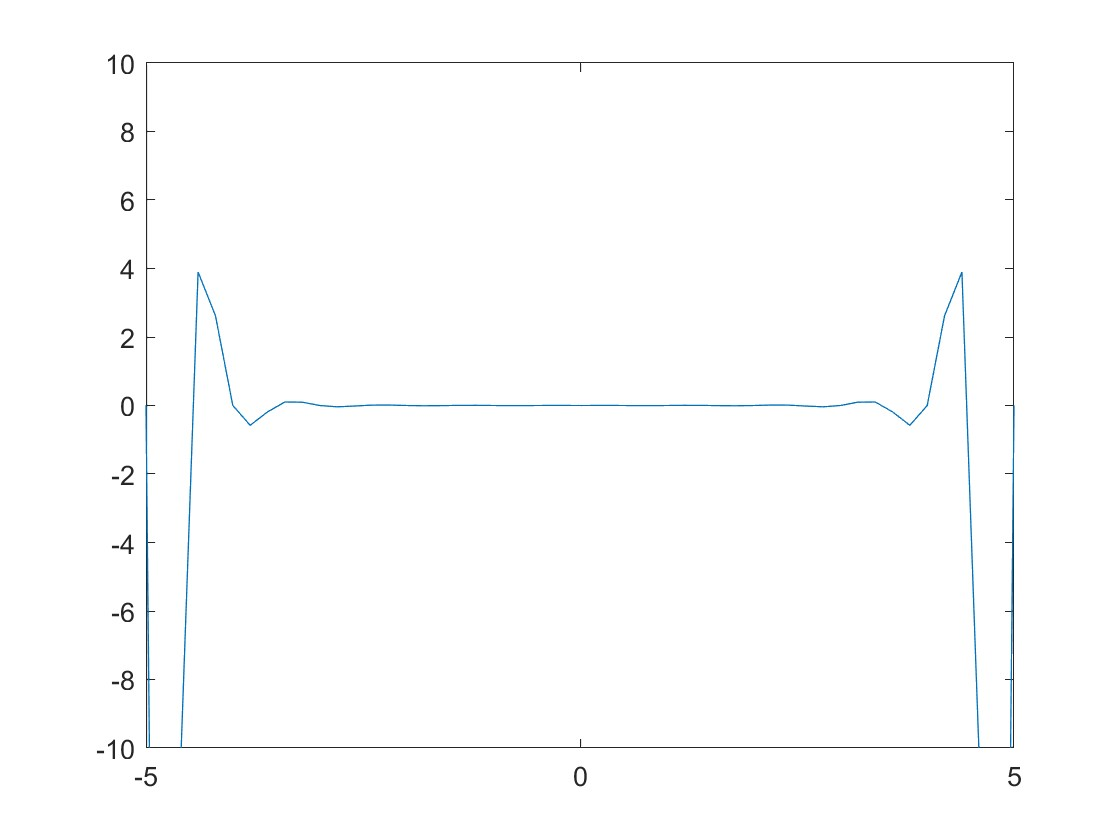
\includegraphics[width=0.9\textwidth]{assignment_2_4_fig.jpg}
        \centering
        \caption{Plotting of $P(x)-f(x)$}
    \end{figure}

\end{enumerate}


\end{document}